\documentclass[10pt,a4paper,final]{article}
\usepackage[pdftex]{graphicx}
\usepackage[utf8]{inputenc}
\usepackage{amsmath}
\usepackage{amsfonts}
\usepackage{amssymb}
\usepackage{gensymb}
%\usepackage{tikz}
\usepackage{empheq}
\usepackage{booktabs}
\usepackage{multirow}


\title{Model for elastic energy of a dissociated dislocation}

\begin{document}
\section{Introduction}
\begin{figure}[hbp]
\centering
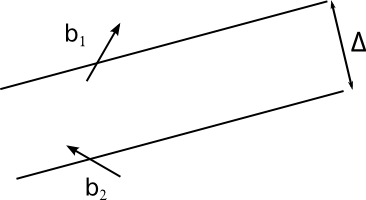
\includegraphics[scale=0.8]{png/parallel_disloc.png}
\caption{General representation of two parallel dislocation segments separated by a distance $\Delta$}
\end{figure}
The general model for the elastic energy per unit length for a mixed dislocation dissociated into two partials can be given as \cite{bacon78}:
\begin{equation}
E_D(\theta) = E_S(\theta) + E_I(\theta,\Delta) + E_F(\Delta,\gamma) \label{eqbacon}
\end{equation}
"$E_S$" is the self-energy, "$E_I$" is the interaction energy, and "$E_F$" is the fault-energy. "$\theta$" is the angle between the Burgers vector and the unit line vector, $\Delta$ is the separation between two line segments, $\gamma$ is the stacking-fault energy.\\

A general expression can be given for each energy.
\begin{subequations}
\begin{align}
E_S(\theta) & = \frac{\mu b^2}{4\pi(1-\nu)}\left(1-\nu\cos^2\theta\right)\ln\left(\frac{R}{r_0}\right) \label{eq:ltmodel}\\
E_I(\theta) & = \frac{\mu b^2}{2\pi}\left(\alpha+\frac{\beta}{1-\nu}\right)\ln\left(\frac{R}{\Delta}\right)-\frac{\mu}{2\pi(1-\nu)}\psi \label{eq:defEi}\\
E_F & = \gamma \Delta \label{eq:defEf}
\end{align}
\end{subequations}
$r_0$ and $R$ are the inner and outer cutoff radii, respectively. $\mu$, $b$, and $\nu$ are the shear modulus, the Burgers vector of the dislocation, and the Poisson ratio.\\

Equation \ref{eq:defEi} is the interaction energy between two parallel dislocation segments separated by a vector $\vec{\Delta}$. $\alpha$, $\beta$, and $\psi$ are related to the Burgers vectors and the line direction vectors of the two dislocations. $\Delta$ is the vector pointing from one dislocation segment to the second.

$\gamma$ is the stacking-fault energy

\section{Interaction energy between two parallel in-plane dislocation segments}
The interaction energy between two parallel dislocations is defined from eq.(5-16)\cite{hirth1982theory}. It has the same form as defined in eq.(\ref{eq:defEi}). As such $\alpha$, $\beta$, and $\psi$ are defined as:
\begin{subequations}
\begin{align}
\alpha &= \left(\vec{b}_1 \cdot \hat{l}\right)\left(\vec{b}_2 \cdot \hat{l}\right) \\
\beta &= \left(\vec{b}_1 \wedge \hat{l}\right) \cdot \left(\vec{b}_2 \wedge \hat{l}\right) \\
\psi &= \frac{1}{\Delta^2}\left[\left(\vec{b}_1 \wedge \hat{l}\right) \cdot \vec{\Delta}\right]
\left[\left(\vec{b}_2 \wedge \hat{l}\right) \cdot \vec{\Delta}\right]
\end{align}
\label{eq:alphabeta}
\end{subequations}
For our case, the dislocations also exist in the same plane since they are partials. Hence $\vec{b}_i \wedge \hat{l} \perp \vec{\Delta} \Rightarrow \psi = 0$ for our model. \\ 

The form of the elastic energy is then

\begin{subequations}
\begin{align*}
E_D(\theta) &= E_S(\theta) + E_I(\theta,\Delta) + \gamma\Delta \\
 &= E_S(\theta) + \frac{\mu}{2\pi}\left(\alpha+\frac{\beta}{1-\nu}\right)\ln\frac{R}{\Delta} + \gamma\Delta
\end{align*}
\end{subequations}
Taking the partial derivative wrt $\Delta$ to find the equilibrium separation $d$
\begin{subequations}
\begin{align*}
\left.\frac{\partial E_D}{\partial\Delta}\right|_{\Delta=d} &= \frac{\mu}{2\pi}\left(\alpha+\frac{\beta}{1-\nu}\right)\frac{-1}{d} + \gamma \\
0 &= \frac{\mu}{2\pi}\left(\alpha+\frac{\beta}{1-\nu}\right)\frac{-1}{d} + \gamma \\
\end{align*}
\end{subequations} 

Which gives the relation between the equilibrium separation and the interaction energy coefficients

\begin{equation}
\gamma d = \frac{\mu}{2\pi}\left(\alpha+\frac{\beta}{1-\nu}\right) \label{eq:gammad}
\end{equation}

Replacing equation \ref{eq:gammad} in equation \ref{eqbacon} we get the general form

\begin{equation}
\boxed{
E_D(\theta) = E_S(\theta+\phi) + E_S(\theta-\phi) + \gamma d \ln\frac{R}{d} + \gamma d} \label{eq:finalED}
\end{equation}

%%%%%%%%%%%%%%%%%%%%%%%%%%%% Shockley dislocation
\section{Shockley dislocation ($\theta, \phi=\pm\pi/6$)}
\begin{figure}[hbtp]
\centering
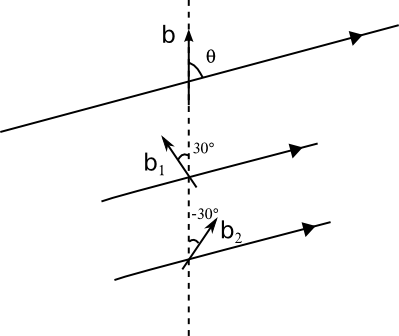
\includegraphics[scale=1]{png/shockley_schema.png}
\caption{Representation of a Shockley pair}
\end{figure}

\subsection{Self-energy}
Using equation (\ref{eq:ltmodel}) we can show that the self-energy for a pair of Shockley partials is given as
\begin{equation}
E_S\left(\theta+\frac{\pi}{6}\right) + E_S\left(\theta-\frac{\pi}{6}\right) \cong 2 - \nu\cos^2\left(\theta+\frac{\pi}{6}\right) - \nu\cos^2\left(\theta-\frac{\pi}{6}\right) \label{eq:self1shoc}
\end{equation}

Using the identity: 
\begin{equation}
\cos^2(A+B) + \cos^2(A-B) = 2(\cos^2A\cos^2B + \sin^2A\sin^2B) \label{eqcosplus}
\end{equation}

And letting $A = \theta, B = \pi/6$ we get
\begin{subequations}
\begin{align*}
\cos^2\left(\theta+\frac{\pi}{6}\right) + \cos^2\left(\theta-\frac{\pi}{6}\right) &= 
2\left(\frac{3}{4}\cos^2\theta + \frac{1}{4}\sin^2\theta \right) \\
&= \frac{1}{2}(3\cos^2\theta + \sin^2\theta) \\
&= \frac{1}{2}(1+2\cos^2\theta)
\end{align*}
\end{subequations}

Replacing in equation \ref{eq:self1shoc} gives:
\begin{equation}
\begin{split}
E_S\left(\theta+\frac{\pi}{6}\right) + E_S\left(\theta-\frac{\pi}{6}\right) &=
\frac{\mu b^2}{4\pi}\ln\left(\frac{R}{r_0}\right)\frac{1}{1-\nu}\left[2-\frac{\nu}{2}(1+2\cos^2\theta)\right] \\
&=\frac{\mu b^2}{8\pi}(4-\nu-2\nu\cos^2\theta)\ln\frac{R}{r_0} \label{eq:e_self_shockley}
\end{split}
\end{equation}

\subsection{Interaction energy}
Hirth \cite{hirth1982theory}(eq.10-15) defines the equilibrium separation between two Shockley partials as:
\begin{equation}
\gamma_B d_B = \frac{\mu b^2}{8\pi}\frac{2-\nu}{1-\nu}\left(1-\frac{2\nu\cos2\theta}{2-\nu}\right)
\label{eq:hirth1015}
\end{equation}

\subsection{Full expression}
Replacing equations \ref{eq:hirth1015} and \ref{eq:e_self_shockley} in equation \ref{eq:finalED} we get the elastic energy of a pair of Shockley partial dislocations
\begin{equation}
\begin{split}
E_D^B(\theta,\nu,\gamma) &= \frac{\mu b^2}{8\pi}\frac{4-\nu-2\cos^2\theta}{1-\nu}\ln\frac{R}{r_0} \\ 
&+\frac{\mu b^2}{8\pi}\left(1-\frac{2\nu\cos2\theta}{2-\nu}\right)\left(\ln\frac{R}{d_B} + 1 \right)
\end{split}
\label{eq:EDshoc}
\end{equation}
where $d_B$ is defined in equation \ref{eq:hirth1015}.

%%%%%%%%%%%%%%%%%%%% Prismatic pair
\section{Prismatic dislocation ($\theta, \phi= 0)$}
\begin{figure}[hbtp]
\centering
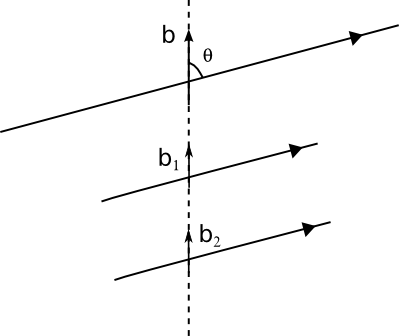
\includegraphics[scale=1]{png/prism_schema.png}
\caption{Representation of a prismatic pair}
\end{figure}
\subsection{Self-energy}
The self energy of a pair of dislocations with equal Burgers vectors ($\phi=0$) is just double that for a single
\begin{equation}
E_S(\theta) = 2\cdot\frac{\mu b^2}{4\pi}\frac{1-\nu\cos^2\theta}{1-\nu}\ln\frac{R}{r_0} \label{eq:selfprism}
\end{equation}

\subsection{Interaction energy}
There is no equation in \cite{hirth1982theory} similar to that of \ref{eq:hirth1015}, so we will derive it here.
The equilibrium separation between the pair of dislocations in the prismatic plane can be obtained from equation \ref{eq:alphabeta}

\begin{subequations}
\begin{align*}
\alpha &= b^2\cos^2\theta \\
\beta &= b^2\sin^2\theta
\end{align*}
Replacing in equation \ref{eq:gammad} gives
\begin{align*}
\gamma d &= \frac{\mu b^2}{2\pi}\left(\cos^2\theta+\frac{\sin^2\theta}{1-\nu}\right) \\
&= \frac{\mu b^2}{2\pi}\frac{1}{1-\nu}(\cos^2\theta -\nu\cos^2\theta +\sin^2\theta ) \\
&= \frac{\mu b^2}{2\pi}\frac{1}{1-\nu}(1 - \nu\cos^2\theta) \\
&= \frac{\mu b^2}{2\pi}\frac{1}{1-\nu}\left(1 - \nu\frac{\cos2\theta+1}{2}\right) \\
&= \frac{\mu b^2}{4\pi}\frac{1}{1-\nu}(2 - \nu\cos2\theta - \nu) \\
\end{align*}
And we get
\begin{equation}
\gamma_Pd_P = \frac{\mu b^2}{4\pi}\frac{2-\nu}{1-\nu}\left(1 - \frac{\nu\cos2\theta}{2-\nu}\right) \label{eq:gdprism}
\end{equation}
\end{subequations}
which is quite similar to equation \ref{eq:hirth1015} up to the constant inside the paranthases. 

\subsection{Full expression}
If we combine equations \ref{eq:gdprism} and \ref{eq:selfprism} we get
\begin{equation}
\begin{split}
E_D^P(\theta, \nu, \gamma) &=  \frac{\mu b^2}{4\pi}\frac{2}{1-\nu}(1-\nu\cos^2\theta)\ln\frac{R}{r_0} \\
&+\frac{\mu b^2}{4\pi}\frac{2-\nu}{1-\nu}\left(1-\frac{\nu\cos2\theta}{2-\nu}\right)\left(\ln\frac{R}{d_P} + 1\right)
\end{split}
\label{eq:EDprism}
\end{equation}
where $d_P$ is defined in equation \ref{eq:gdprism}.

\section{Implementation for the case of Zr}
We will take $E_0 = [\mu a^2/\pi] = [\text{J/m}]$ as units of energy and $a$ as units of distance. 

\begin{table}[hb]
\centering

\begin{tabular}{ll} \toprule
Paramter & value \\ \midrule
$\mu$ (GPa) & 34 \\
$\lambda$ (GPa) & 131.143 \\
$\nu$ & 0.3970 \\
a (\AA) & 3.232 \\
$\gamma_{\text{prism}}$ (mJ/m$^2$) & 135 \\
$\gamma_{\text{basal}}$ (mJ/m$^2$) & 198 \\ 
$R$ (A) & 1000 \\
$r_0$ (A) & 1 \\
\bottomrule
\end{tabular}
\end{table}

This gives the following results:

\begin{table}[hbt]
\centering
\begin{tabular}{llccc|cc} \toprule
& & $E_{S}$ & $E_I+E_F$ & $d_\text{eq}$ & $E_D$ & $1-E^\text{s}_D/E^\text{e}_D$ \\ \midrule
\multirow{2}{*}{prism} & screw & 0.8635 & 0.6949 & 3.239 & 1.5584 & \multirow{2}{*}{0.3716}\\ & edge & 1.3408 & 0.37714 & 0.9874 & 2.480 & \\ 
\rule{0pt}{4ex} \multirow{2}{*}{basal} & screw & 1.341 & 0.37714 & 5.372 & 1.7180 & \multirow{2}{*}{0.35355} \\ & edge & 1.720 & 0.0.93773 & 2.9264 & 2.6576 & \\ 
\bottomrule

\end{tabular}

\end{table}

We note that the screw dislocation ($\theta=0$) in the prismatic plane (green curve) has the lowest energy. The energy difference between the screw dislocation in the basal and the prismatic plane is roughly $\Delta_{PB}(\theta=0) = 0.1596 ~\frac{\mu a^2}{\pi} = 0.3538 ~\text{eV/\AA}$ (300 K $\approx$ 26 meV).

\begin{figure}[htbp]
\centering
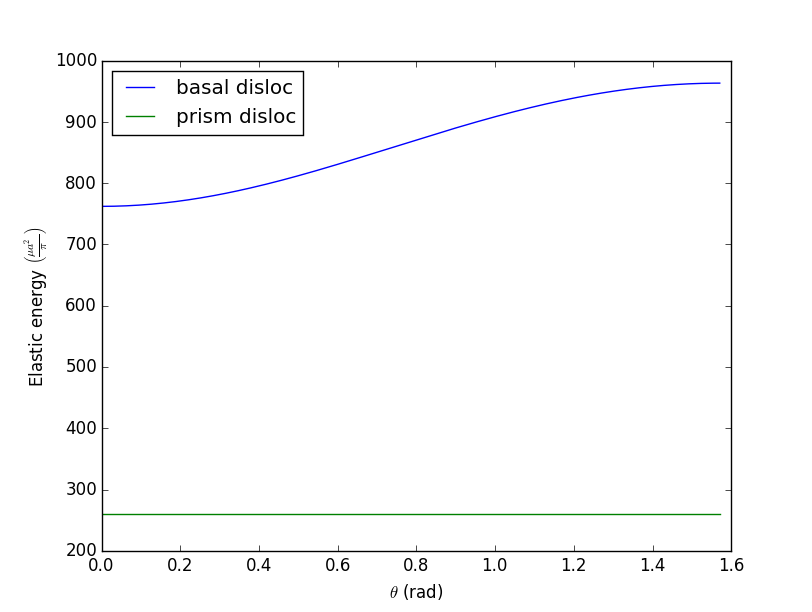
\includegraphics[scale=0.7]{png/zr_basal_prism}
\caption{Dislocation self-energy taking into account dissociation effects (bacon-line-tension model) as a function of dislocation character. Case of zirconium $b=1/3\left<11\bar{2}0\right>$}
\label{fig:zr}
\end{figure}
\pagebreak
\section{Cross-slip of basal segment}
We want to determine in this section the critical angle for which a basal segment is able to cross-slip into the prismatic plane and remain stable. We use the elastic energy per unit length determined in the previous sections to determine this angle. The approximation to the critical angle therefore neglects interactions between the segments in the two glide planes.\\

\begin{figure}[hbp]
\centering
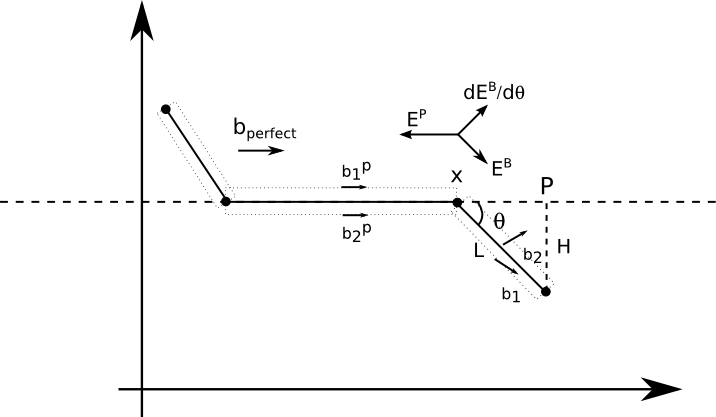
\includegraphics[scale=1]{png/node_schema.png}
\label{fig:crossslip}
\end{figure}

Consider for example the configuration shown in figure \ref{fig:crossslip}. We want to calculate the fornce on node 3. There are two sources of force: the force due to the prismatic section ($\theta=0$) and due to the rotated basal section ($\theta$). $\theta$ defined in this configuration is equivalent to the $\theta$ used in the definition of the elastic energy per unit length (equations \ref{eq:EDshoc} and \ref{eq:EDprism}). \\
The force in both cases is equal to 
\begin{equation}
F^{P/B}_x = -\frac{d E_T}{d x} = -\frac{d}{d x}\left(L^{P/B}E^{P/B}(\theta)\right) \label{eq:Fxpb}
\end{equation}

\subsection{Force from prismatic}
Using equation \ref{eq:Fxpb} and $L^P = x$
\begin{equation}
F^{P}_x = -\frac{d}{d x}\left(xE^P_D(0)\right) = -E^P_D(0)
\label{eq:FxP}
\end{equation}

\subsection{Force from basal}
Using equation \ref{eq:Fxpb} we find
\begin{equation*}
F_x^B = -\frac{d}{dx}\left(L E_D(\theta)^B\right)
\end{equation*}
Using the chain rule we change variables $x(\theta,L)$
\begin{equation*}
\frac{d}{dx} = \frac{d\theta}{dx}\frac{\partial}{\partial\theta} + \frac{dL}{dx}\frac{\partial}{\partial L}
\end{equation*}
Using $\tan\theta = (P-x)/H$
\begin{align*}
P-x &= \frac{H}{\tan\theta} \\
-dx &= -\frac{H}{\sin^2\theta} \\
\frac{d\theta}{dx} &= \frac{\sin^2\theta}{H} \\
\frac{d\theta}{dx} &= \frac{\sin\theta}{L}
\end{align*}  
We also find for $L$
\begin{align*}
(P-x)^2 + H^2 &= L^2 \\
-2(P-x)dx &= 2LdL \\
\frac{dL}{dx} &= -\frac{P-x}{L} \\
\frac{dL}{dx} &= -\cos\theta
\end{align*}
Hence we can now write
\begin{equation}
\frac{d}{dx} = \frac{sin\theta}{L}\frac{\partial}{\partial\theta} - \cos\theta\frac{\partial}{\partial L} \label{eq:chainx}
\end{equation}

Hence using equation \ref{eq:chainx} and \ref{eq:Fxpb}

\begin{equation*}
F_x^B = -\left(\frac{sin\theta}{L}\frac{\partial}{\partial\theta} - \cos\theta\frac{\partial}{\partial L}\right)\left(LE_D^B(\theta)\right)
\end{equation*}
\begin{equation}
F_x^B = -\sin\theta\frac{\partial E_D^B(\theta)}{\partial\theta} + \cos\theta E_D^B(\theta) \label{eq:FxB}
\end{equation}

The condition for the stability of the node connecting the two dislocation segments can now be given as $F_x^P = F_x^B$ which using equations \ref{eq:FxB} and \ref{eq:FxP} is:

\begin{equation}
\boxed{ \cos\theta E_D^B(\theta) - \sin\theta\frac{\partial E_D^B(\theta)}{\partial\theta} = E_D^P(\theta=0) } \label{eq:nodecond}
\end{equation}

We plot the equation \ref{eq:nodecond} in \ref{fig:nodestab} and we find the root of the equation using numerical methods. We show that the critical angle $\theta_c = 0.2406~\text{rad} = 13.785 \degree$. For all angles below that the sum of forces is positive (positive direction of motion see figure \label{fig:fig:crossslip}), and the prismatic dislocation is stable.

\begin{figure}
\centering
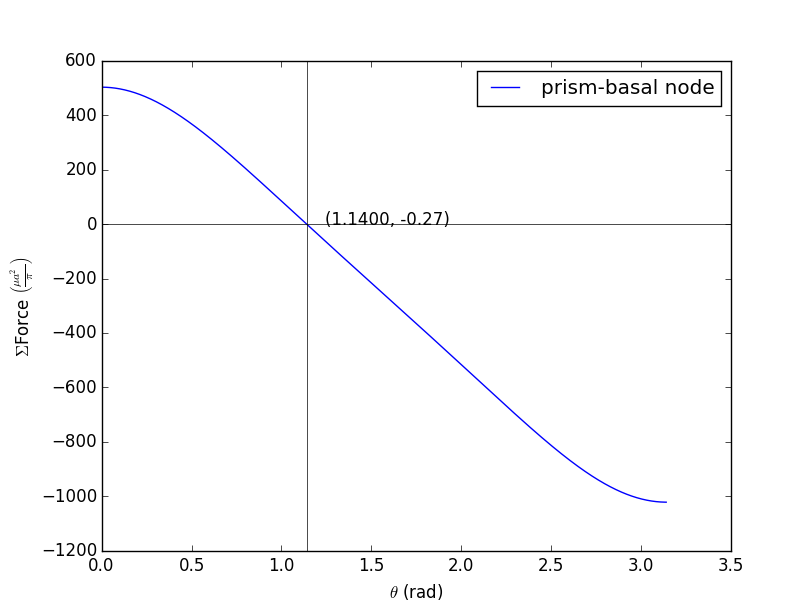
\includegraphics[scale=0.6]{png/force_node.png}
\caption{Sum of forces on node connecting a prismatic screw dislocation and a mixed basal dislocation in Zr}
\label{fig:nodestab}
\end{figure}
\pagebreak

\section{Implementation in NUMODIS}
We want to implement the previous model in NUMODIS. The model needs to function for any type of dislocation in any crystal structure; however, to test it we will report results for zirconium only. We use the files "linetension.C", "linetension.h", and "linetension.hpp" to write the code for our model.

\begin{description}
\item[baconlinetension.h] Is an empty file.
\item[baconlinetension.C] Contains the declaration of a COREENERGY mode so that the class can be constructed from a keyword.
\item[baconlinetension.hpp] Contains the definitions of the main functions of the model: \texttt{ComputeForce} and \texttt{ComputeEnergy}
\end{description}
\textbf{Warning!} Unlike \texttt{linetension}, \texttt{baconlinetension} is implemented only for a \texttt{GSystem}.

\subsection{Expression for energy}
The most general expression for the energy using this model is given in equation \ref{eq:finalED}. The total energy for a segment with unit vector $\hat{\xi}$, length $\xi$, and dissociated burgers vectors $\vec{b}_1$ and $\vec{b}_2$ is given as
\begin{equation}
\begin{split}
E_T &= \xi\cdot\frac{\mu b_1^2}{4\pi(1-\nu)}\left[1-\nu(\hat{b}_1\cdot\hat{\xi})^2\right]\log\left(\frac{R}{r0}\right) + \xi\cdot\frac{\mu b_2^2}{4\pi(1-\nu)}\left[1-\nu(\hat{b}_2\cdot\hat{\xi})^2\right]\log\left(\frac{r0}{R}\right) \\
 & ~~ + \xi\cdot\gamma d\log\frac{R}{d} \\
 & ~~ + \xi\cdot\gamma d
\end{split}
\label{eq:computeenergy}
\end{equation}
where
\begin{equation}
\begin{split}
\gamma d &= \frac{\mu}{2\pi} \left[ \left(\vec{b}_1\cdot\hat{\xi}\right)\left(\vec{b}_2\cdot\hat{\xi}\right) + \frac{\left(\vec{b}_1\times\hat{\xi}\right)\cdot\left(\vec{b}_2\times\hat{\xi}\right)}{1-\nu}\right] \\
&= \frac{\mu}{2\pi(1-\nu)}
\left[ \left(\vec{b}_1\cdot\hat{\xi}\right)\left(\vec{b}_2\cdot\hat{\xi}\right)(1-\nu) + \left(\vec{b}_1\cdot\vec{b}_2\right)\left(\hat{\xi}\cdot\hat{\xi}\right) - \left(\vec{b}_1\cdot\hat{\xi}\right)\left(\hat{\xi}\cdot\vec{b}_2\right)\right] \\
&= \frac{\mu}{2\pi(1-\nu)} \left[\left(\vec{b}_1\cdot\vec{b}_2\right) - \nu\left(\vec{b}_1\cdot\hat{\xi}\right)\left(\vec{b}_2\cdot\hat{\xi}\right)\right] \\
&= \frac{\mu b_1b_2}{2\pi(1-\nu)}\left[\left(\hat{b}_1\cdot\hat{b}_2\right) - \nu\left(\hat{b}_1\cdot\hat{\xi}\right)\left(\hat{b}_2\cdot\hat{\xi}\right)\right]
\end{split}
\label{eq:gammadnumodis}
\end{equation}
\subsection{Expression for force}
The force acting on node 1 $F_i$ is given by the derivative of the energy with respect to $\xi_i$. The derivative of the first line in equation \ref{eq:computeenergy} is already given by the line-tension model in \texttt{linetension.hpp:117}
\begin{equation}
\vec{F}_{\text{lt}} = E_0\left[1+\nu\left(\hat{b}\cdot\hat{\xi}\right)\right]\hat{\xi} - 2E_0\nu\left(\hat{b}\cdot\hat{\xi}\right)\hat{b}
\label{eq:computeforcelt}
\end{equation}
where $E_0 = \frac{\mu b^2}{4\pi(1-\nu)}\log\frac{R}{r_0}$\\

We will now find the derivative of the second and third line of equation \ref{eq:computeenergy} with the help of equation \ref{eq:gammadnumodis}

\begin{equation*}
\begin{split}
\gamma d &= \frac{\mu b_1b_2}{2\pi(1-\nu)} \left[\left(\hat{b}_1\cdot\hat{b}_2\right)-\nu\frac{\left(b_{1x}\xi_{x}+b_{1y}\xi_{y}+b_{1z}\xi_{z}\right)\left(b_{2x}\xi_{x}+b_{2y}\xi{y}+b_{2z}\xi_{z}\right)}{b_1b_2\left(\xi_x^2+\xi_y^2+\xi_z^2\right)}\right]\\
\frac{\partial\gamma d}{\partial\xi_x} &= -F_0\nu\left\lbrace \frac{b_{1x}\left(\vec{b}_2\cdot\vec{\xi}\right) + b_{2x}\left(\vec{b}_1\cdot\vec{\xi}\right)}{\left(b_1b_2\xi^2\right)^2}b_1b_2\xi^2
 -\frac{2\xi_xb_1b_2}{\left(b_1b_2\xi^2\right)^2}\left(\vec{b}_1\cdot\vec{\xi}\right)\left(\vec{b}_2\cdot\vec{\xi}\right) \right\rbrace \\
 &= -F_0\nu\left\lbrace \frac{1}{\xi}\frac{\vec{b}_2\cdot\vec{\xi}}{b_2\xi}\frac{b_{1x}}{b_1} + \frac{1}{\xi}\frac{\vec{b}_1\cdot\vec{\xi}}{b_1\xi}\frac{b_{2x}}{b_2}
 -2\frac{\left(\vec{b}_1\cdot\vec{\xi}\right)\left(\vec{b}_2\cdot\vec{\xi}\right)}{b_1b_2\xi^2}\frac{\xi_xb_1b_2}{\xi^2b_1b_2}\right\rbrace \\
 &= -F_0\nu\left\lbrace \frac{1}{\xi}\left(\hat{b}_2\cdot\hat{\xi}\right)\frac{b_{1x}}{b_1} + \frac{1}{\xi}\left(\hat{b}_1\cdot\hat{\xi}\right)\frac{b_{2x}}{b_2} - 2\frac{1}{\xi}\left(\hat{b}_1\cdot\hat{\xi}\right)\left(\hat{b}_2\cdot\hat{\xi}\right)\frac{\xi_x}{\xi} \right\rbrace
\end{split}
\end{equation*}
where $F_0 = \frac{\mu b_1b_2}{2\pi(1-\nu)}$
Which implies that
\begin{equation}
\frac{\partial\gamma d}{\partial\xi_i} = 
-\frac{F_0\nu}{\xi}\left\lbrace  
\left(\hat{b}_2\cdot\hat{\xi}\right)\hat{b}_1 + 
\left(\hat{b}_1\cdot\hat{\xi}\right)\hat{b}_2 - 
2\left(\hat{b}_1\cdot\hat{\xi}\right)\left(\hat{b}_2\cdot\hat{\xi}\right)\hat{\xi}
\right\rbrace
\label{eq:forcegammad}
\end{equation}
We can now write the complete expression for the dissociated-line tension
\begin{equation*}
\begin{split}
\vec{F}_{bacon} &= \vec{F}_\text{lt}(\vec{b}_1) + \vec{F}_\text{lt}(\vec{b}_2) + 
\frac{\partial}{\partial \xi_i}\left[\xi \gamma d \ln\frac{R}{d} + \gamma d\xi\right]\\
&= \vec{F}_\text{lt}(\vec{b}_1) + \vec{F}_\text{lt}(\vec{b}_2) +
\left(\gamma d\ln\frac{R}{d} + \gamma d\right)\hat{\xi} + 
\frac{\partial\gamma d}{\partial\xi_i}\ln\frac{R}{d}\xi +
\frac{\xi\gamma d}{d}\frac{\partial d}{\partial\xi_i} +
\xi\frac{\partial\gamma d}{\partial\xi_i}
\end{split}
\end{equation*}
Hence,
\begin{equation}
\boxed{\vec{F}_{bacon} = \vec{F}_\text{lt}(\vec{b}_1) + \vec{F}_\text{lt}(\vec{b}_2) +
\gamma d\left(1+\ln\frac{R}{d}\right)\hat{\xi} + \left(2+\ln\frac{R}{d}\right)\xi\frac{\partial \gamma d}{\partial \xi_i}}
\label{eq:forcebaconlt}
\end{equation}
\bibliography{bacon78.bib,hirth82}
\bibliographystyle{plain}
\end{document}



